% Case 2 causal DAG -- from pub_rse_methodology/formalization_short.tex
% RS transforms the research context: new variables AND new interpretations.
\documentclass[tikz,border=6pt]{standalone}
% Shared preamble for the standalone renders of the RIGHT-framework figures.
% The tikz styles are copied verbatim from pub_rse_methodology/uml_shapes.tex so
% that the standalone PDFs look exactly like the ones in the paper.
\usepackage[utf8]{inputenc}
\usepackage[T1]{fontenc}
\usepackage{graphicx}
\usepackage{times}
\usepackage{amssymb}
\usepackage{xcolor}
\usepackage{tikz}
\usetikzlibrary{arrows.meta,positioning,shapes.geometric,shapes.misc,calc}

\tikzset {
    initial/.style={circle, fill=black, minimum size=5mm, inner sep=0pt},
    action/.style={draw, rounded corners=2pt, minimum width=28mm,
        minimum height=8mm, align=center},
    decision/.style={draw, diamond, aspect=2, minimum height=8mm,
        minimum width=8mm, inner sep=1pt, align=center},
    fork/.style={draw, fill=black, minimum width=20mm, minimum height=4mm},
    vfork/.style={draw, fill=black, minimum width=2mm, minimum height=14mm},
    box/.style={draw, rounded corners=2mm, thick, minimum width=18mm,
        minimum height=8mm, align=center},
    rsepic/.style={inner sep=0pt, outer sep=2pt},
    dependency/.style={dashed, <->},
    node distance=8mm,
    uml_activity/.style={draw, line width=0.6pt,
        -{Straight Barb[angle=40:5pt 5]}},
    >=Latex,
    every path/.style={uml_activity}
}

\newcommand{\terminus}{
\includegraphics[height=6mm]{uml_endnode.png}}
\newcommand{\rsecycle}{
\includegraphics[height=12mm]{rse-cycle.png}}

\begin{document}
    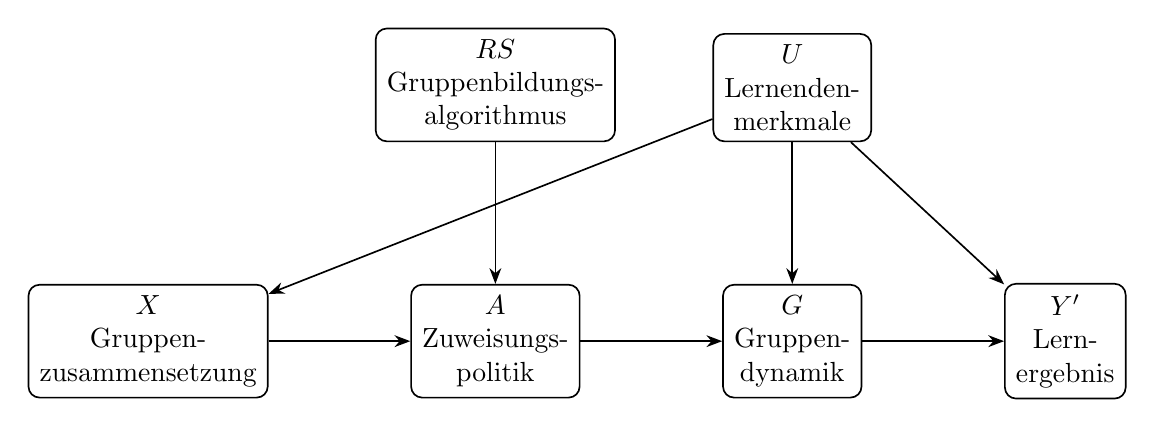
\begin{tikzpicture}[>=Stealth, node distance=18mm]

        \tikzstyle{node}=[draw, rounded corners, align=center, inner sep=4pt,
            every path/.style={shorten >=2pt, shorten <=2pt}]

        \node[node] (RS) {$RS$\\Gruppenbildungs-\\algorithmus};
        \node[node, below=of RS] (A) {$A$\\Zuweisungs-\\politik};
        \node[node, left=of A] (X) {$X$\\Gruppen-\\zusammensetzung};
        \node[node, right=of A] (G) {$G$\\Gruppen-\\dynamik};
        \node[node, right=of G] (Yp) {$Y'$\\Lern-\\ergebnis};
        \node[node, above=of G] (U) {$U$\\Lernenden-\\merkmale};

        \draw[->] (RS) -- (A);
        \draw[->] (X) -- (A);
        \draw[->] (A) -- (G);
        \draw[->] (G) -- (Yp);
        \draw[->] (U) -- (G);
        \draw[->] (U) -- (Yp);
        \draw[->] (U) -- (X);

    \end{tikzpicture}
\end{document}
